108. а) $\cfrac{(x^2+4x+3)(x-1)}{x+1}=\cfrac{(x+1)(x+3)(x-1)}{x+1}=x^2+2x-3,\ x
eq-1.$
$$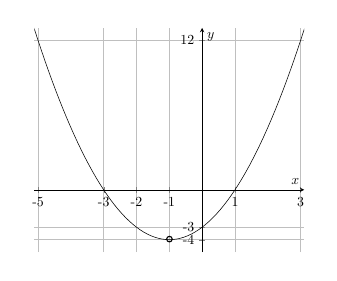
\begin{tikzpicture}[scale=0.5]
\begin{axis}[
    axis lines = middle,
    grid=major,
    legend pos={south west},
    xlabel = {$x$},
    ylabel = {$y$},
    ymin=-5,
    ymax=13,
    xtick={-5, -3, -2, -1, 1, 3},
    xticklabels={-5, -3, -2, -1, 1, 3},
    ytick={-4, -3,12},
    yticklabels={-4, -3,12}             ]
	\addplot[domain=-6:5, samples=100, color=black] {x*x+2*x-3};
%\addplot[domain=-3.1:2.5, samples=100, color=red] {70*abs(1-2*abs(abs(x)-2))-10*x^2+10*x-70};
	%\addlegendentry{$\text{Рис. 1}$};
\end{axis}
\draw (3.43,0.33) circle (2pt);
\end{tikzpicture}$$
б) По графику определим, что функция принимает значения $(-4;-3].$\\
